El presente manual proporciona una guía básica para que los nuevos usuarios puedan comenzar a utilizar la aplicación ``LogArt: Galería de Recuerdos'' y aprovechar sus funcionalidades principales.

\section{Acceso a la Aplicación}
\label{appB:acceso}
Para acceder a LogArt, abra su navegador web y diríjase a la URL donde la aplicación ha sido desplegada (\ref{appA:ejecucionApp}).
\begin{itemize}
    \item \textbf{Página de Inicio (Hero):} Si no ha iniciado sesión, verá la página de inicio, que presenta información general sobre LogArt y una sección de Preguntas Frecuentes (FAQs). Desde aquí, podrá optar por registrarse o iniciar sesión. Figura \ref{fig:pantallaHero}

    \begin{figure}
   \centering

  \begin{minipage}{0.45\textwidth}
   \centering

     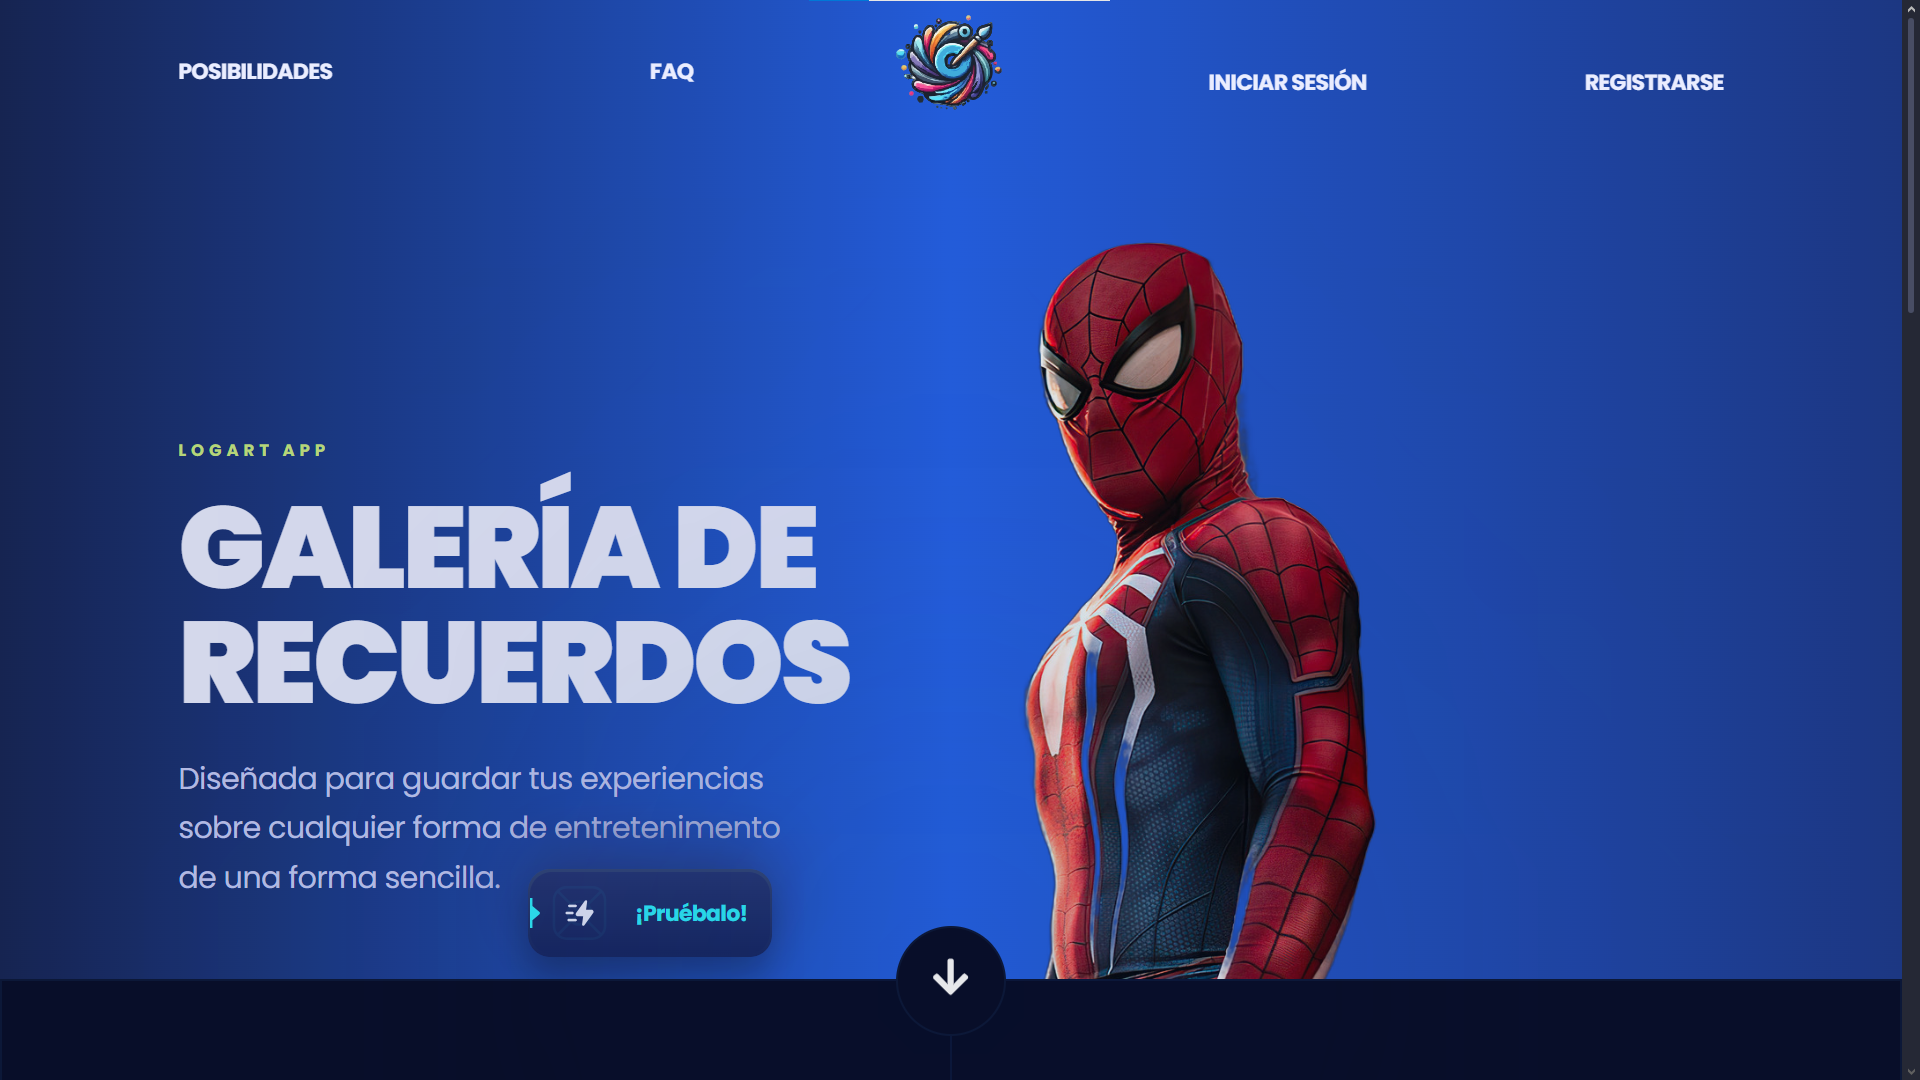
\includegraphics[clip=true,width=\textwidth]{img/hero1home.png}\\

    \footnotesize (g)
  \end{minipage}
  \caption{Pantalla Hero (home).}\label{fig:pantallaHero}
  \end{figure}
  
    \item \textbf{Usuarios Anónimos:} Como usuario no registrado, puede explorar los objetos que otros usuarios hayan decidido compartir públicamente, siempre y cuando tenga el link disponible. Figura \ref{fig:pantallaObjetoDetalle}
\end{itemize}

\section{Registro de una Nueva Cuenta}
\label{appB:registro}
Para utilizar todas las funcionalidades de LogArt, como crear sus propias galerías y objetos, necesitará registrarse. Figura \ref{fig:pantallaRegistro}
\begin{enumerate}
    \item En la página de inicio o desde el menú de navegación, haga clic en la opción "Registrarse".
    \item Complete el formulario de registro proporcionando:
    \begin{itemize}
        \item Nombre de Usuario.
        \item Nombre.
        \item Apellidos.
        \item Dirección de Correo Electrónico (válida).
        \item Contraseña.
    \end{itemize}
    \item Tras enviar el formulario, recibirá un correo electrónico en la dirección proporcionada con un enlace para verificar su cuenta.
    \item Haga clic en el enlace de verificación en el correo para activar su cuenta. Este paso es obligatorio para poder iniciar sesión.
\end{enumerate}
\begin{figure}
   \centering

  \begin{minipage}{0.45\textwidth}
   \centering

     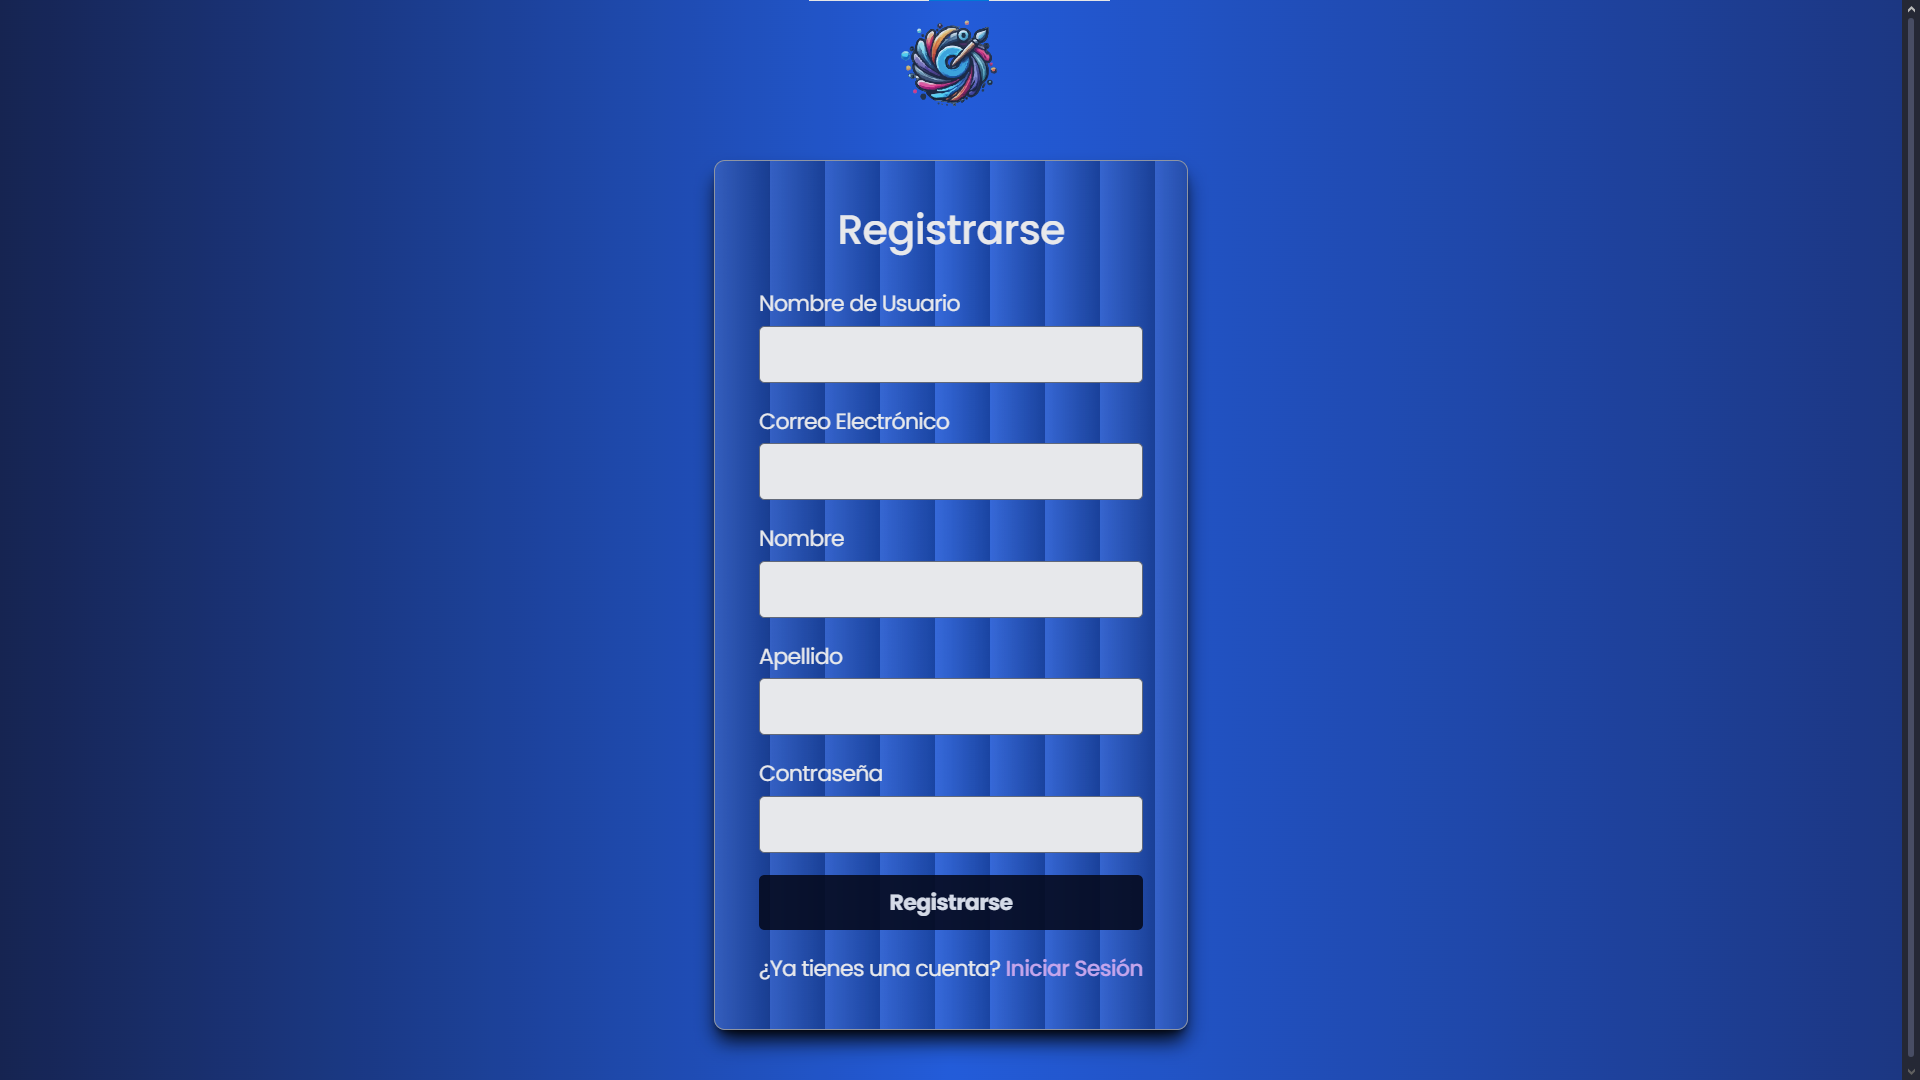
\includegraphics[clip=true,width=\textwidth]{img/register.png}\\

    \footnotesize (h)
  \end{minipage}
  \caption{Pantalla Registro.}\label{fig:pantallaRegistro}
  \end{figure}

\section{Inicio de Sesión}
\label{appB:inicioSesion}
Una vez que su cuenta esté verificada: Figura \ref{fig:pantallaLogin}
\begin{enumerate}
    \item Haga clic en la opción ``Iniciar Sesión'' (Login) desde la página de inicio, o en el menú de navegación.
    \item Ingrese su correo electrónico y la contraseña con la que se registró.
    \item Si las credenciales son correctas, accederá a su panel personal de LogArt.
\end{enumerate}
\textbf{Recuperación de Contraseña:} Si olvida su contraseña, puede utilizar la opción ``¿Olvidaste tu contraseña?'' en la página de inicio de sesión para iniciar el procedimiento de restablecimiento a través de su correo electrónico. Figura \ref{fig:pantallaLogin}

\begin{figure}
   \centering

  \begin{minipage}{0.45\textwidth}
   \centering

     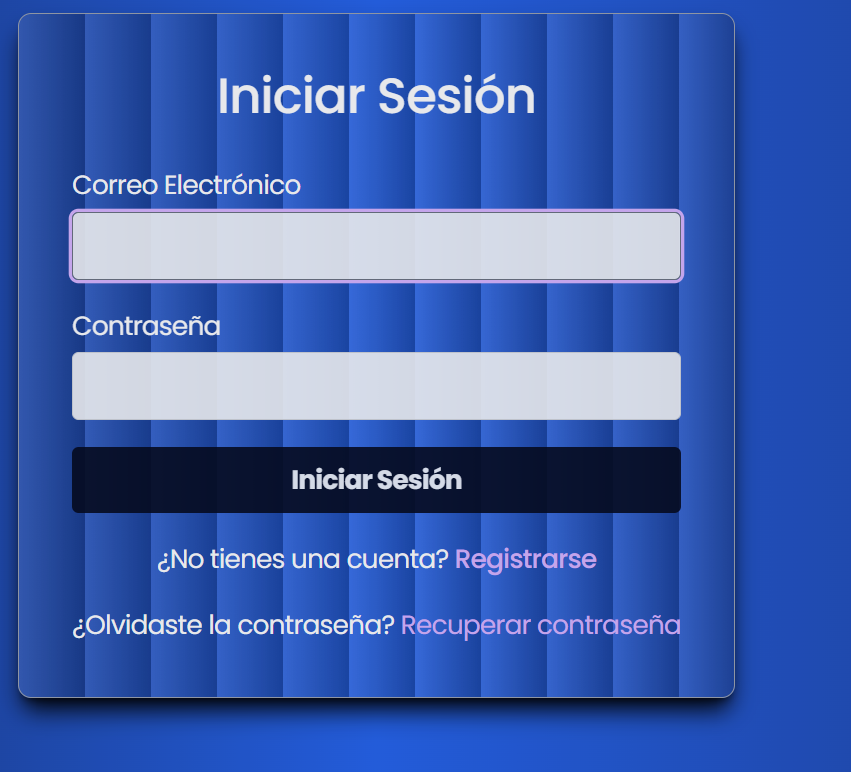
\includegraphics[clip=true,width=\textwidth]{img/pass1.png}\\

    \footnotesize (i)
  \end{minipage}
  \caption{Pantalla de Inicio de Sesión.}\label{fig:pantallaLogin}
  \end{figure}

\section{Navegación Principal y Galerías}
\label{appB:navegacionGalerias}
Una vez iniciada la sesión: Figura \ref{fig:pantallaGaleria}
\begin{itemize}
    \item \textbf{Selección de Disciplina:} Se le presentará la pantalla de galerías, con un selector para seleccionar una disciplina (Libros, Canciones, Videojuegos) para acceder a su galería personal correspondiente. Puede cambiar entre estas galerías de diferentes disciplinas utilizando el mismo selector.
    \item \textbf{Vista de Galería:} Muestra todos los objetos que ha creado para la disciplina seleccionada. Puede buscar objetos por nombre o filtrar para ver solo sus favoritos. Si tiene muchos objetos, la galería se mostrará paginada.
\end{itemize}


\section{Gestión de Objetos}
\label{appB:gestionObjetos}
\begin{itemize}
    \item \textbf{Crear un Nuevo Objeto:}
    \begin{enumerate}
        \item En la vista de galería, haga clic en el botón verde ``Crear Objeto''. Figura \ref{fig:pantallaGaleria}
        \item Se abrirá un formulario modal donde deberá ingresar:
        \begin{itemize}
            \item Nombre del objeto.
            \item Descripción.
            \item Disciplina.
            \item Una imagen representativa para el objeto.
        \end{itemize}
        \item Haga clic en ``Crear'' para guardar el objeto en su galería.
    \end{enumerate}
    \item \textbf{Ver Detalles de un Objeto:} Haga clic en el nombre o la imagen de un objeto en la galería para acceder a su vista detallada. Aquí verá toda su información y los comentarios asociados. Figura \ref{fig:pantallaObjetoDetalle}
    \item \textbf{Editar un Objeto:} Si es el propietario del objeto, en la tarjeta del objeto encontrará una opción para ``Editar''. Esto abrirá un formulario similar al de creación para modificar sus datos. \ref{fig:pantallaGaleria}
    \item \textbf{Eliminar un Objeto:} Si es el propietario del objeto, podrá eliminar un objeto desde su tarjeta en la galería, con un botón similar al de ``Editar'', pero con el texto ``Eliminar'' y en rojo. Se le pedirá confirmación antes de la eliminación. Figura \ref{fig:pantallaGaleria}
\end{itemize}

\begin{figure}
   \centering

  \begin{minipage}{0.45\textwidth}
   \centering

     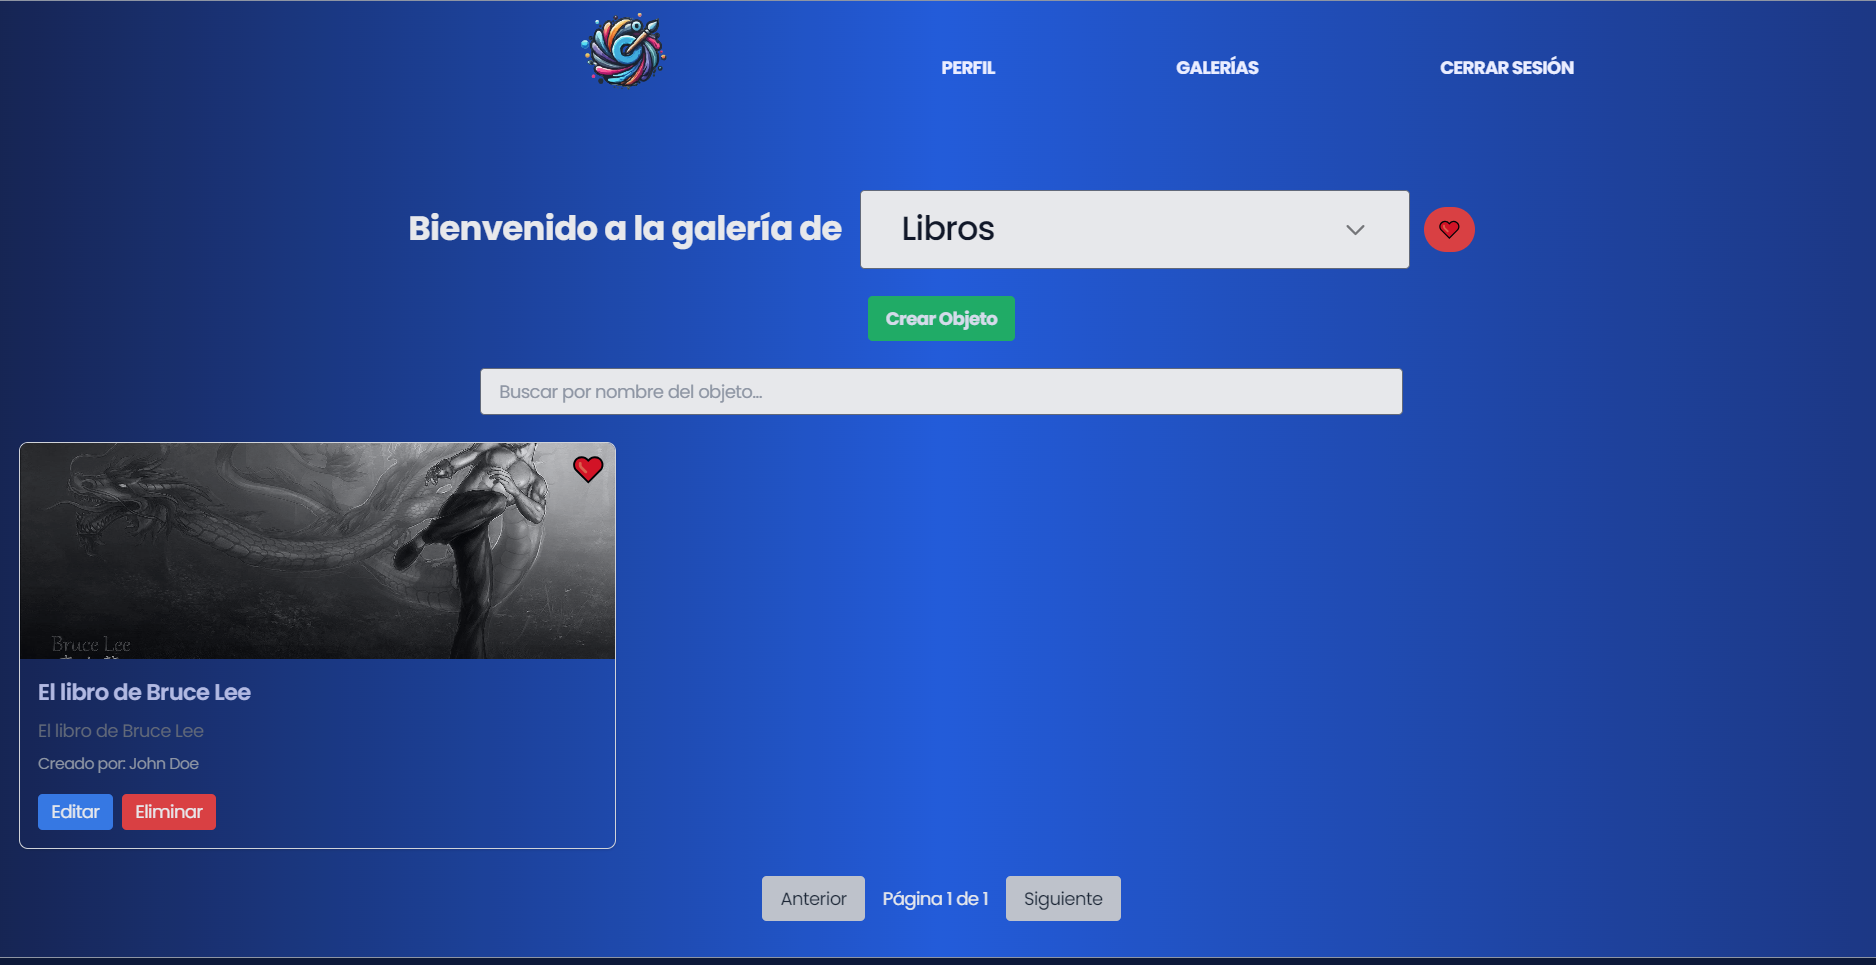
\includegraphics[clip=true,width=\textwidth]{img/fav2.png}\\

    \footnotesize (j)
  \end{minipage}
  \caption{Pantalla de Galería de Objetos.}\label{fig:pantallaGaleria}
  \end{figure}

\section{Gestión de Comentarios}
\label{appB:gestionComentarios}
Los comentarios le permiten añadir sus recuerdos y experiencias detalladas a cada objeto.
\begin{itemize}
    \item \textbf{Añadir un Comentario:} En la vista detallada de un objeto de su propiedad, encontrará una sección para escribir y guardar nuevos comentarios.
    \item \textbf{Editar / Eliminar Comentarios:} Si es el autor del comentario, o un administrador, podrá editar su contenido o eliminarlo.
\end{itemize}

\begin{figure}
   \centering

  \begin{minipage}{0.45\textwidth}
   \centering

     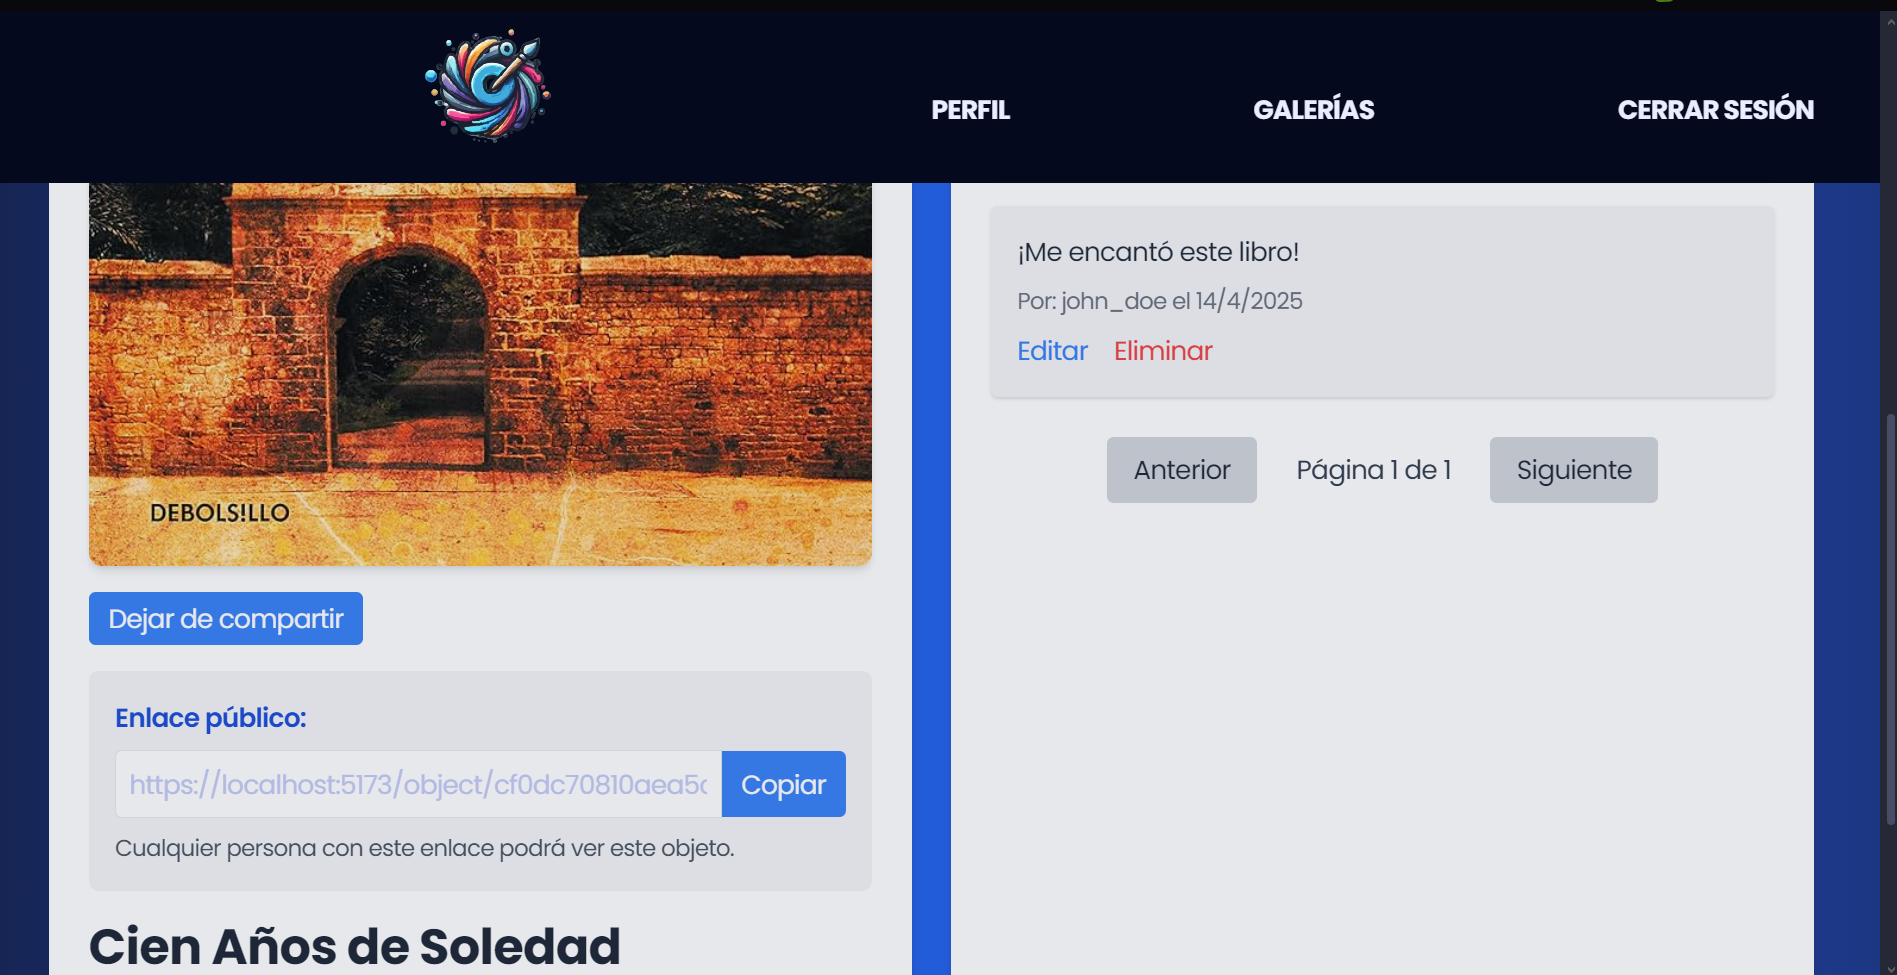
\includegraphics[clip=true,width=\textwidth]{img/share2.png}\\

    \footnotesize (k)
  \end{minipage}
  \caption{Pantalla de Objeto en Detalle.}\label{fig:pantallaObjetoDetalle}
  \end{figure}

\section{Funcionalidades Adicionales menores para Usuarios Registrados}
\label{appB:funcionalidadesAdicionales}
\begin{itemize}
    \item \textbf{Compartir Objetos:} Puede optar por hacer públicos sus objetos para que otros usuario, incluso no registrados, puedan verlos. Esta opción está disponible en la vista detallada del objeto. Al compartir, se genera un enlace único. Figura \ref{fig:pantallaObjetoDetalle}
    \item \textbf{Marcar como Favorito:} En la tarjeta de cada objeto, encontrará un icono de un corazón para marcar o desmarcar un objeto como favorito, facilitando su acceso posterior mediante el filtro de favoritos. Figura \ref{fig:pantallaGaleria}
    \item \textbf{Gestión de Perfil:} Desde el menú de navegación, puede acceder a su ``Perfil'' para actualizar su nombre, apellido, usuario, imagen de perfil y biografía.
\end{itemize}

\section{Panel de Administración (Solo para Administradores)}
\label{appB:panelAdmin}
Los usuarios con rol de administrador tienen acceso a un ``Panel de Administración'' o \textit{Dashboard} desde el menú principal. Este panel ofrece: Figura \ref{fig:pantallaDashboard}
\begin{itemize}
    \item Estadísticas sobre el uso de la plataforma (usuarios, contenido, actividad, crecimiento).
    \item Herramientas para visualizar y moderar (eliminar) todos los objetos y comentarios (una vez dentro de los objetos) de la plataforma.
    \item Una vista para gestionar usuarios.
\end{itemize}

\begin{figure}
   \centering

  \begin{minipage}{0.45\textwidth}
   \centering

     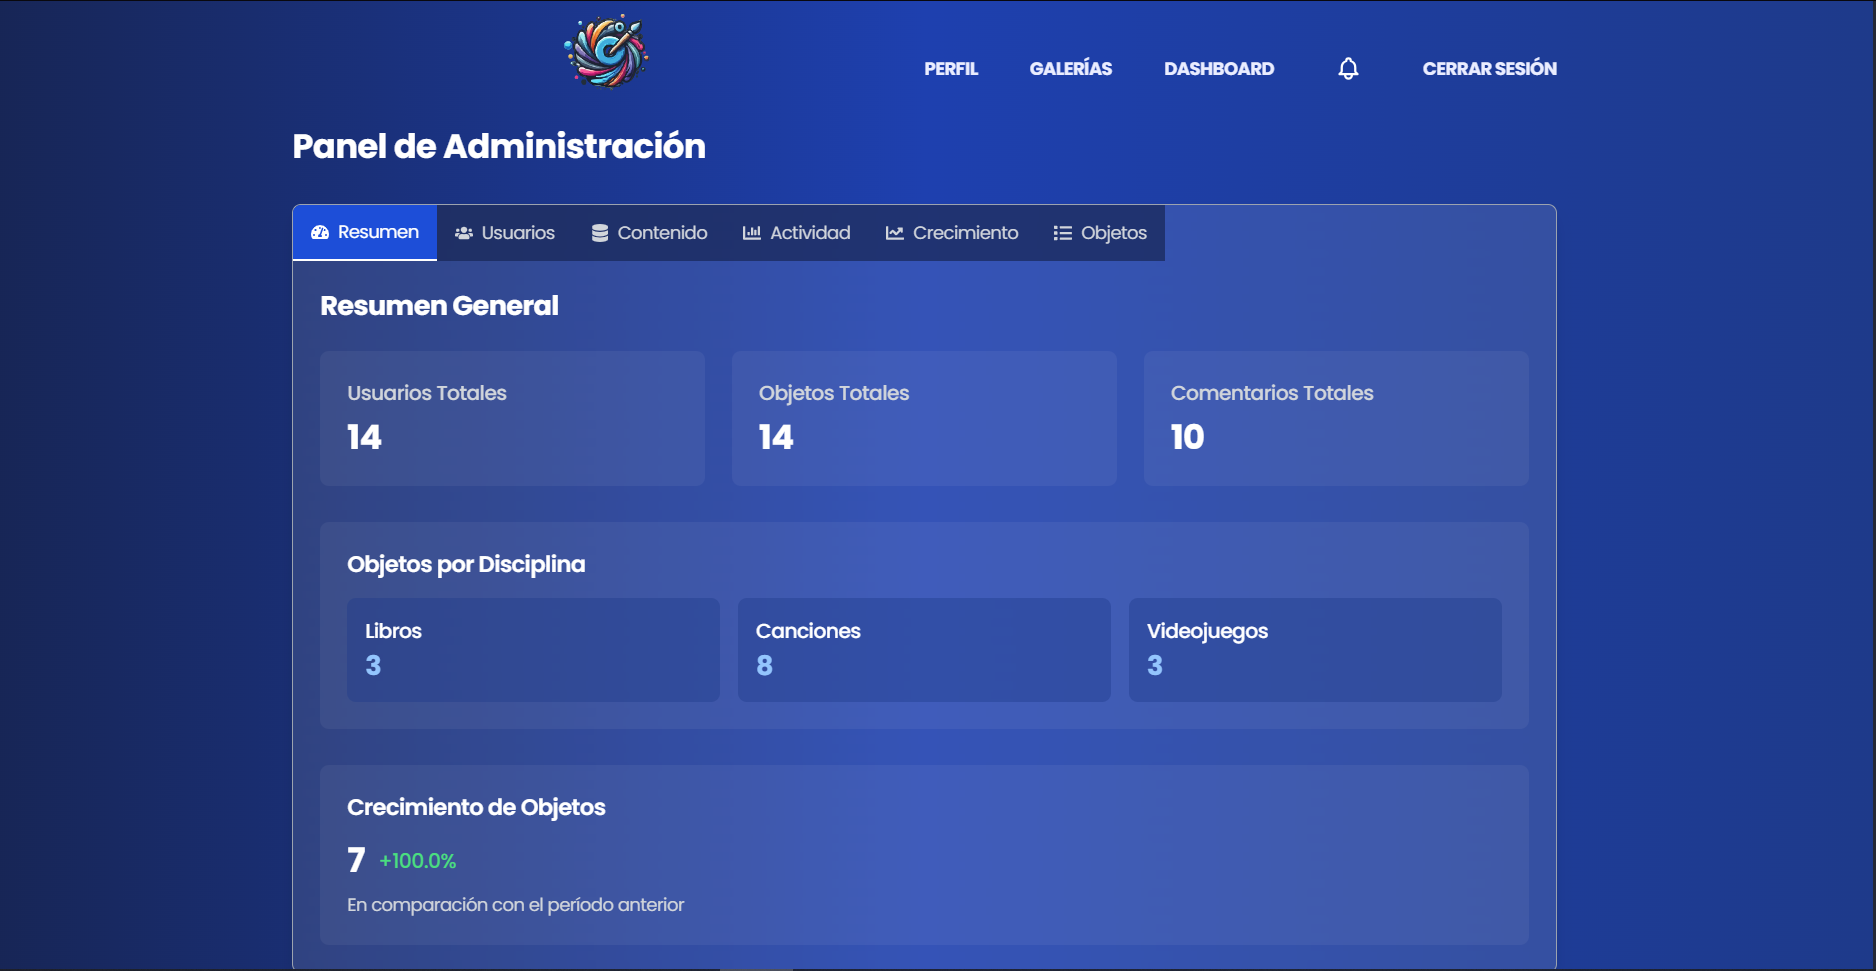
\includegraphics[clip=true,width=\textwidth]{img/dashboard2.png}\\

    \footnotesize (l)
  \end{minipage}
  \caption{Pantalla de Dashboard de Administrador.}\label{fig:pantallaDashboard}
  \end{figure}
  
El funcionamiento detallado de cada sección del dashboard es intuitivo y se presenta a través de diferentes pestañas, además de estar claramente definido en \ref{rf:adminFuncionalidades}

\section{Cierre de Sesión}
\label{appB:cierreSesion}
Para finalizar su sesión en LogArt, utilice la opción ``Cerrar Sesión'' disponible en el menú de navegación
